\documentclass[preprint,12pt]{elsarticle}
\usepackage{amsmath,amssymb}
\usepackage{graphicx}
\usepackage{booktabs}
\emergencystretch=2em
\usepackage{hyperref}
\usepackage{xurl}
\usepackage{listings}
\usepackage{xcolor}
\usepackage{tikz}
\usetikzlibrary{positioning,arrows.meta,fit}
\lstset{basicstyle=\ttfamily\small,columns=fullflexible,frame=single,breaklines=true}
\graphicspath{{../../results/figures/}}

\journal{SoftwareX}

\begin{document}
\begin{frontmatter}

\title{analogue-risk: a fast, leakage-safe engine for regime-conditioned analogue forecasting of financial risk}

\author[cse]{Manas Ganesh Dasari\corref{cor1}}
\ead{bl.sc.u4cse24229@bl.students.amrita.edu}
\author[cse]{Vishal KVS}
\author[math]{K. N. Meera}
\cortext[cor1]{Corresponding author}
\affiliation[cse]{organization={Department of Computer Science and Engineering, Amrita School of Computing, Amrita Vishwa Vidyapeetham},
  city={Bengaluru}, country={India}}
\affiliation[math]{organization={Department of Mathematics, Amrita School of Computing, Amrita Vishwa Vidyapeetham},
  city={Bengaluru}, country={India}}

\begin{abstract}
Nearest-neighbour ("analogue") forecasting is attractive in finance because every forecast can be
traced to concrete historical episodes, yet published evaluations are often vulnerable to
look-ahead bias, overlapping samples and backtest overfitting. \texttt{analogue-risk} is an
open-source Rust engine with Python bindings that makes such evaluations fast and leakage-safe.
It provides regime-conditioned $k$-nearest-neighbour and Gaussian-kernel analogue forecasters
over arbitrary causal features and targets, an exclusion zone that keeps analogue outcome
windows independent, a Markov-mixture over volatility regimes, a trade simulator shared between
label construction and backtesting, Hawkes and GARCH likelihoods, and a complete walk-forward
evaluation suite: Diebold--Mariano tests, the model confidence set, VaR/ES backtests, deflated
Sharpe ratios and pre-registered hypothesis tests. A full-history analogue search over 200,000
bars runs in about 90 seconds on a laptop, and every table of the accompanying study is
reproduced by a single command.
\end{abstract}

\begin{keyword}
analogue forecasting \sep nearest neighbours \sep volatility forecasting \sep value-at-risk \sep
Hawkes process \sep backtesting \sep Rust \sep reproducibility
\end{keyword}
\end{frontmatter}

%% ------------------------------------------------------------------
\section*{Code metadata}
\begin{table}[h]
\footnotesize
\begin{tabular}{p{0.05\linewidth}p{0.38\linewidth}p{0.49\linewidth}}
\toprule
Nr. & Code metadata description & \\
\midrule
C1 & Current code version & v2.0.0 \\
C2 & Permanent link to code/repository & \url{https://github.com/ManasDasri/analogue-risk} \\
C3 & Permanent link to reproducible capsule & -- \\
C4 & Legal code license & MIT \\
C5 & Code versioning system used & git \\
C6 & Software code languages, tools and services used & Rust, Python; PyO3, maturin, rayon; NumPy, SciPy, pandas, scikit-learn, Matplotlib \\
C7 & Compilation requirements, operating environments and dependencies & Python $\geq$3.12 (prebuilt wheels: Linux, macOS, Windows); building from source needs Rust stable \\
C8 & Link to developer documentation/manual & \url{https://github.com/ManasDasri/analogue-risk/blob/main/docs/api.md} \\
C9 & Support email for questions & bl.sc.u4cse24229@bl.students.amrita.edu \\
\bottomrule
\end{tabular}
\end{table}

%% ------------------------------------------------------------------
\section{Motivation and significance}

The method of analogues \cite{lorenz1969,farmer1987} forecasts the future of a system by finding
past states that resemble the present and aggregating what happened next. In finance it has
been used for exchange rates \cite{fernandez1999} and is widely re-implemented in retail trading
tools, where it appeals because it is interpretable: every forecast is backed by a list of
historical episodes a user can inspect. The same features make analogue methods easy to evaluate
wrongly. Three failure modes are common:
(i) \emph{look-ahead}: an analogue whose outcome window has not yet closed at the forecast time
leaks the future;
(ii) \emph{dependent neighbours}: adjacent bars have nearly identical features, so the ``$k$
nearest'' analogues are often one episode counted $k$ times, which makes confidence statements
meaningless; and
(iii) \emph{backtest overfitting}: many configurations are tried and the best is reported
\cite{bailey2014,harvey2016}.

\texttt{analogue-risk} grew out of a TradingView strategy that combined a one-dimensional
analogue matcher, a Markov volatility regime, a Poisson crash gate and Kelly sizing. Rebuilding it
to be evaluated properly required an engine that is causal by construction, fast enough to
search the \emph{entire} history at every bar, and paired with the statistical tooling that
forecasting and finance journals expect. No existing open-source package combines these. The
software makes three contributions: a leakage-safe, parallel analogue engine; a label/execution
design in which the same trade simulator scores historical analogues and live trades; and an
end-to-end, pre-registrable evaluation pipeline. The accompanying study \cite{dasari_research}
uses it to show, across 24 assets, that analogue methods carry no directional information but
produce well-calibrated, competitive risk forecasts.

%% ------------------------------------------------------------------
\section{Software description}

\subsection{Software architecture}
The package is a Rust crate compiled to a Python extension module (\texttt{analogue\_risk.\_core}) with PyO3
and maturin, plus a thin Python layer (Fig.~\ref{fig:arch}). All per-bar work is in Rust and
releases Python's global interpreter lock; per-bar forecasts are independent and run in parallel
with rayon.

\begin{figure}[t]
\centering
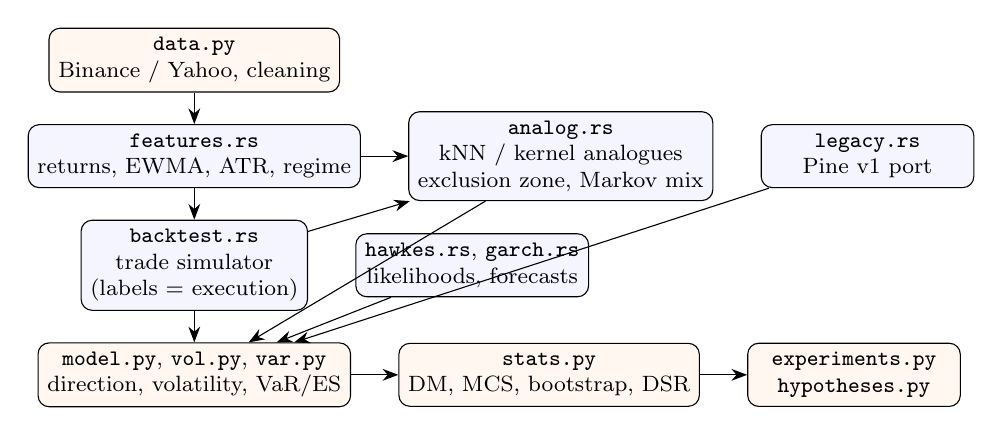
\begin{tikzpicture}[node distance=4mm and 6mm, every node/.style={font=\footnotesize},
  box/.style={draw, rounded corners, align=center, minimum width=27mm, minimum height=8mm, fill=blue!4},
  py/.style={box, fill=orange!6}, arr/.style={-{Stealth[length=2mm]}}]
\node[py] (data) {\texttt{data.py}\\Binance / Yahoo, cleaning};
\node[box, below=of data] (feat) {\texttt{features.rs}\\returns, EWMA, ATR, regime};
\node[box, right=of feat] (analog) {\texttt{analog.rs}\\kNN / kernel analogues\\exclusion zone, Markov mix};
\node[box, below=of feat] (bt) {\texttt{backtest.rs}\\trade simulator\\(labels = execution)};
\node[box, right=of bt] (hg) {\texttt{hawkes.rs}, \texttt{garch.rs}\\likelihoods, forecasts};
\node[box, right=of analog] (leg) {\texttt{legacy.rs}\\Pine v1 port};
\node[py, below=of bt] (models) {\texttt{model.py}, \texttt{vol.py}, \texttt{var.py}\\direction, volatility, VaR/ES};
\node[py, right=of models] (stats) {\texttt{stats.py}\\DM, MCS, bootstrap, DSR};
\node[py, right=of stats] (exp) {\texttt{experiments.py}\\\texttt{hypotheses.py}};
\draw[arr] (data) -- (feat); \draw[arr] (feat) -- (analog); \draw[arr] (feat) -- (bt);
\draw[arr] (bt) -- (analog); \draw[arr] (bt) -- (models); \draw[arr] (analog) -- (models);
\draw[arr] (hg) -- (models); \draw[arr] (leg) -- (models); \draw[arr] (models) -- (stats); \draw[arr] (stats) -- (exp);
\end{tikzpicture}
\caption{Architecture. Blue: Rust core; orange: Python layer.}
\label{fig:arch}
\end{figure}

\subsection{Software functionalities}

\paragraph{Analogue engine} At bar $t$ a causal embedding $x_t\in\mathbb{R}^m$ is compared with
every past anchor $j$ whose targets $y_j\in\mathbb{R}^p$ are fully observed ($j\le t-\delta$ for a
declared delay $\delta$). In $k$NN mode the nearest anchors are accepted greedily, per volatility
regime, subject to an exclusion zone ($|j-j'|\ge e$ for all accepted $j,j'$), so outcome windows
of length $h\le e$ never overlap. A partial selection (\texttt{select\_nth\_unstable}) followed by a
full sort only when needed keeps this near $O(n)$ per bar. Regime groups are combined with the
$h$-step forecast of a two-state Markov chain estimated from prefix transition counts in $O(1)$
per bar, giving $\hat y_t=\sum_s \pi_s(t)\,\bar y_s(t)$ with standard errors of the mixture mean.
A Gaussian-kernel mode (Nadaraya--Watson \cite{nadaraya1964,watson1964}) weights all candidates
and reports Kish effective sample sizes \cite{kish1965}. \texttt{neighbours()} returns the index
and weight of every analogue, so any functional of the analogue distribution (quantiles, expected
shortfall, explanations such as Fig.~\ref{fig:explain}) can be computed. A configuration guard
rejects settings in which the exclusion zone would force non-neighbours into the set.

\paragraph{Labels equal execution} \texttt{backtest.rs} simulates a trade (next-open fill,
intrabar stop-before-target, gap fills, time stop, costs). The same function computes the
R-multiple label of every historical anchor, so a forecaster is trained on exactly the event
the strategy executes; a test asserts bit-level agreement.

\paragraph{Benchmarks and risk models} EWMA \cite{riskmetrics1996}, GARCH(1,1) \cite{bollerslev1986}
by maximum likelihood, HAR \cite{corsi2009}, gradient boosting \cite{friedman2001,pedregosa2011},
exponential Hawkes processes \cite{hawkes1971} with an exact $O(n)$ likelihood, historical and
filtered historical simulation \cite{baroneadesi1999}, and analogue-conditioned VaR/ES.

\paragraph{Evaluation} Walk-forward folds in which every fitted quantity sees only earlier data;
QLIKE \cite{patton2011}; Diebold--Mariano tests \cite{diebold1995} with Newey--West variance
\cite{newey1987}; the model confidence set \cite{hansen2011} with the stationary bootstrap
\cite{politis1994}; Kupiec \cite{kupiec1995} and Christoffersen \cite{christoffersen1998} coverage
tests and the Fissler--Ziegel FZ0 loss \cite{fissler2016,patton2019}; probabilistic and deflated
Sharpe ratios \cite{bailey2012,bailey2014}; and a pre-registered hypothesis module with Holm
correction \cite{holm1979}.

\paragraph{Public API and data} \texttt{Analogue} exposes the engine with named, validated
options and labelled outputs; \texttt{volatility\_forecast(prices, horizon)} is a one-call risk
forecaster. Every series used in the study is pinned (last bar, row count, SHA-256), so re-runs
reproduce the published numbers or warn that a source has changed; Binance data fall back to the
public bulk archive where the API is geo-blocked.

\paragraph{Quality assurance} Thirty-six Python and twelve Rust tests cover causality (forecasts,
labels and the legacy port are identical when all data after $t$ is removed), likelihoods against
brute force, Hawkes parameter recovery, recovery of a planted signal versus a random walk,
known-answer checks of every backtest and statistic, and a regression test that reproduces the
pre-registered hypothesis tables. CI runs them on Linux, macOS and Windows with Python 3.12 and 3.13
and enforces formatting; tagged releases build wheels for all three platforms. An executable
harness compares the legacy port with TradingView's own trade list.

%% ------------------------------------------------------------------
\section{Illustrative examples}

Listing~\ref{lst:ex} forecasts next-day volatility of the S\&P 500 with analogues and compares it
with HAR and GARCH under the walk-forward protocol.

\begin{lstlisting}[language=Python, caption={Walk-forward volatility forecasting.}, label={lst:ex}]
from analogue_risk import data, model as M, vol as V, stats as S
from analogue_risk.experiments import split
mkt = M.Market(data.yahoo("^GSPC", start="1927-12-30"))
d = V.VolData(mkt, V.DAILY_W)                   # h = 5 days
cal, folds = split(mkt.n, V.DAILY_W.warmup)
F, _ = V.walk_forward(d, folds)                 # EWMA, GARCH, HAR, GBM, Analogue, Analogue+HAR
ok = (d.realised > 0)
ok[:cal] = False
losses = {k: V.qlike(d.realised[ok], f[ok]) for k, f in F.items()}
print(S.model_confidence_set(losses, B=1000, block=10))
\end{lstlisting}

Three executed tutorials accompany the code: volatility forecasting with
explanations, VaR backtesting, and---to show the engine is not specific to finance---forecasting
the Lorenz system with delay-embedding analogues, where it beats persistence by 72--94\% in RMSE
depending on the horizon. Figure~\ref{fig:explain} shows the interpretability the engine exposes: for a given hour it
returns the historical volatility paths closest to the present and what followed them.

\begin{figure}[t]
\centering
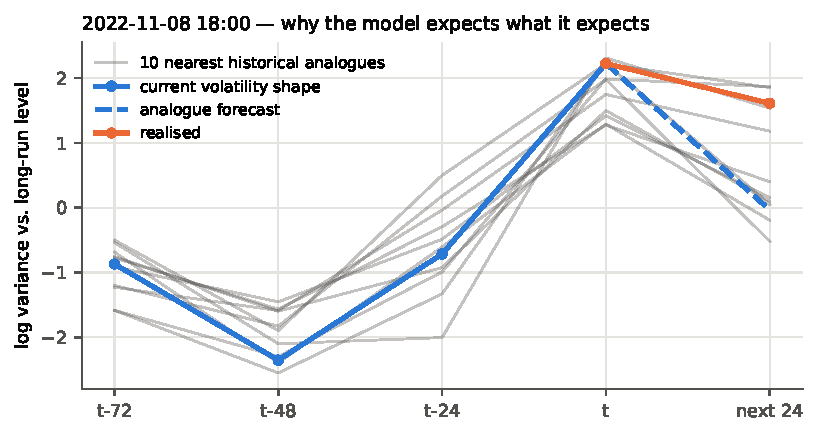
\includegraphics[width=\linewidth]{fig_analogue_explanation.pdf}
\caption{Explaining a forecast: BTC on 8 November 2022. The current volatility shape (blue), its
ten nearest historical analogues (grey) and what followed them, the forecast, and the realised
outcome (orange).}
\label{fig:explain}
\end{figure}

\paragraph{Performance} On an Apple M4 (10 cores) the capped-history $k$NN forecaster processes
about 30,000 bars/s; the full-history search is $O(n^2)$ and forecasts 200,000 bars in about
90\,s; a backtest over 76,000 bars takes about 3\,ms. The complete development study (9 assets,
15 series--horizon pairs, bootstrap inference) runs in about 35 minutes.

%% ------------------------------------------------------------------
\section{Impact}

The engine turned a retail-style trading indicator into a falsifiable research instrument. Its
first use \cite{dasari_research} (i) replicated the original strategy bar-for-bar and showed that
its reported edge does not survive out-of-sample testing with realistic costs; (ii) showed that
analogue forecasts of volatility, combined with HAR, are statistically indistinguishable from the
best standard models, that kernel weighting improves them by 5\%, and that analogue-conditioned VaR
is as well calibrated as filtered historical simulation; and (iii) did so under a public
pre-registration, with the confirmatory analysis code committed before the data it analyses. All
eight pre-registered hypotheses replicated on fifteen assets never used in development.
Because targets and embeddings are arbitrary arrays, the engine applies unchanged to other
analogue problems (other assets, realised measures, macroeconomic series), and its leakage-safe
design and statistical suite lower the cost of evaluating such methods honestly. Researchers can
reproduce every number with one command, and students can inspect every forecast's analogues.

%% ------------------------------------------------------------------
\section{Conclusions}

\texttt{analogue-risk} provides a fast, causal and statistically complete toolkit for analogue
forecasting in finance. Planned extensions are multivariate (cross-asset) analogues, realised
measures from intraday data, and learned combination weights.

\section*{Declaration of competing interest}
The authors hold a patent on the original trading method from which this software was derived.
The software is released under the MIT license.

\section*{Declaration of generative AI and AI-assisted technologies in the writing process}
During the preparation of this work the authors used Claude (Anthropic) to assist with software
development and drafting of the manuscript. After using this tool, the authors reviewed and
edited the content as needed and take full responsibility for the content of the publication.

\bibliographystyle{elsarticle-num}
\bibliography{../refs}

\end{document}
